%%%%%%%%%%%%%%%%%%%%%%%%%%%%%%%%%%%%%%%%%
% Zhovten Games Game Studio Article
% LaTeX Template
% Version 1.7 (April 19, 2026)
%
% This template was created by:
% Vel (enquiries@latextypesetting.com)
% LaTeXTypesetting.com
%
% Modified by Sam Starling (www.linkedin.com/in/sam-starling/, ORCID: https://orcid.org/0009-0009-2621-6372)
%
%!TEX program = xelatex
% Note: this template must be compiled with XeLaTeX rather than PDFLaTeX
% due to the custom fonts used. The line above should ensure this happens
% automatically, but if it doesn't, your LaTeX editor should have a simple toggle
% to switch to using XeLaTeX.
%
%%%%%%%%%%%%%%%%%%%%%%%%%%%%%%%%%%%%%%%%%

%----------------------------------------------------------------------------------------
%	CLASS, PACKAGES AND OTHER DOCUMENT CONFIGURATIONS
%----------------------------------------------------------------------------------------

% Options for packages loaded elsewhere
\PassOptionsToPackage{unicode}{hyperref}
% \PassOptionsToPackage{hyphens}{xurl}
% 
\documentclass{ZGJournalArticle_2026}

\defaultfontfeatures{Scale=MatchLowercase}

\IfFileExists{upquote.sty}{\usepackage{upquote}}{}
\IfFileExists{microtype.sty}{% use microtype if available
  \usepackage[]{microtype}
  \UseMicrotypeSet[protrusion]{basicmath} % disable protrusion for tt fonts
}{}

% A wrapper around soul necessary to make underlining work for Greek.
\usepackage{xesoul}

\usepackage{xcolor}
\usepackage{calc} % for calculating minipage widths
\usepackage[obeyspaces,spaces,hyphens]{xurl}
\urlstyle{same} % Disable monospaced font for ordinary URLs.

% xurl already provides broad line-breaking rules for URLs and paths.
% Do not override \UrlBreaks manually: long path segments may require
% breakpoints beyond '/', '-', '.', and '_'.

\usepackage{fvextra} % Controlled wrapping for verbatim code blocks.

\renewcommand{\floatpagefraction}{.8}%
\setlength{\emergencystretch}{3em} % prevent overfull lines


%----------------------------------------------------------------------------------------
%	PANDOC COMPATIBILITY
%----------------------------------------------------------------------------------------

% Pandoc lists
\providecommand{\tightlist}{%
  \setlength{\itemsep}{0pt}\setlength{\parskip}{0pt}}

% Pandoc tables
% Correct order of tables after \paragraph or \subparagraph.
\usepackage{etoolbox}
\makeatletter
\patchcmd\longtable{\par}{\if@noskipsec\mbox{}\fi\par}{}{}
\makeatother

% Pandoc may emit \def\LTcaptype{none} for captionless longtable blocks.
% Some caption/longtable combinations still look for a counter named `none`.
% Define a dummy counter so uncaptioned Pandoc longtables do not fail.
\makeatletter
\@ifundefined{c@none}{\newcounter{none}}{}
\makeatother

% Allow footnotes in longtable head/foot.
\IfFileExists{footnotehyper.sty}{\usepackage{footnotehyper}}{\usepackage{footnote}}
\makesavenoteenv{longtable}

% Pandoc task lists
% Pandoc may emit \boxtimes / \square for GitHub-style task list checkboxes.
\usepackage{amssymb}

% Pandoc images
\usepackage{graphicx}
\makeatletter
\newsavebox\pandoc@box
\newcommand*\pandocbounded[1]{% scales image to fit in text height/width
  \sbox\pandoc@box{#1}%
  \Gscale@div\@tempa{\textheight}{\dimexpr\ht\pandoc@box+\dp\pandoc@box\relax}%
  \Gscale@div\@tempb{\linewidth}{\wd\pandoc@box}%
  \ifdim\@tempb\p@<\@tempa\p@\let\@tempa\@tempb\fi% select the smaller of both
  \ifdim\@tempa\p@<\p@\scalebox{\@tempa}{\usebox\pandoc@box}%
  \else\usebox{\pandoc@box}%
  \fi%
}
\def\maxwidth{\ifdim\Gin@nat@width>\linewidth\linewidth\else\Gin@nat@width\fi}
\def\maxheight{\ifdim\Gin@nat@height>\textheight\textheight\else\Gin@nat@height\fi}
\makeatother

% Scale images if necessary, so that they will not overflow the page
% margins by default, and it is still possible to overwrite the defaults
% using explicit options in \includegraphics[width, height, ...]{}.
\setkeys{Gin}{width=\maxwidth,height=\maxheight,keepaspectratio}

% Set default figure placement to htbp.
\makeatletter
\def\fps@figure{htbp}
\makeatother

% Pandoc citations
% CSL/citeproc support is kept unconditional here because the build pipeline
% can inject pre-rendered bibliography sections that already contain
% \begin{CSLReferences} ... \end{CSLReferences} even when the final pandoc pass
% itself is executed without --citeproc (for example with suppress-bibliography=true).
% Without these definitions XeLaTeX fails with:
%   LaTeX Error: Environment CSLReferences undefined.
% In other words, the bibliography block is already in the payload, so the
% template must always know how to typeset it.
\NewDocumentCommand\citeproctext{}{}
\NewDocumentCommand\citeproc{mm}{%
  \begingroup\def\citeproctext{#2}\cite{#1}\endgroup}
\makeatletter
% Allow citations to break across lines.
\let\@cite@ofmt\@firstofone
% Avoid brackets around text for \cite.
\def\@biblabel#1{}
\def\@cite#1#2{{#1\if@tempswa , #2\fi}}
\makeatother
\newlength{\cslhangindent}
\setlength{\cslhangindent}{1.5em}
\newlength{\csllabelwidth}
\setlength{\csllabelwidth}{3em}
\newenvironment{CSLReferences}[2] % #1 hanging-indent, #2 entry-spacing
 {\begin{list}{}{% This helps avoid over-stretched lines for DOI links in bibliography.
  \sloppy
  \setlength{\itemindent}{0pt}
  \setlength{\leftmargin}{0pt}
  \setlength{\parsep}{0pt}
  % Turn on hanging indent if param 1 is 1.
  \ifodd #1
   \setlength{\leftmargin}{\cslhangindent}
   \setlength{\itemindent}{-1\cslhangindent}
  \fi
  % Set entry spacing.
  \setlength{\itemsep}{#2\baselineskip}}}
 {\end{list}}
\newcommand{\CSLBlock}[1]{\linebreak \hfill\break\parbox[t]{\linewidth}{\strut\ignorespaces#1\strut}}
\newcommand{\CSLLeftMargin}[1]{\parbox[t]{\csllabelwidth}{\strut#1\strut}}
\newcommand{\CSLRightInline}[1]{\parbox[t]{\linewidth - \csllabelwidth}{\strut#1\strut}}
\newcommand{\CSLIndent}[1]{\hspace{\cslhangindent}#1}

% Pandoc code highlighting
% Required when fenced code blocks are converted to LaTeX with highlighting enabled.
% Defines environments/macros such as Shaded, Highlighting, NormalTok, KeywordTok, etc.
\usepackage{color}
\usepackage{fancyvrb}
\newcommand{\VerbBar}{|}
\newcommand{\VERB}{\Verb[commandchars=\\\{\}]}
\DefineVerbatimEnvironment{Highlighting}{Verbatim}{commandchars=\\\{\}}
% Add ',fontsize=\small' for more characters per line
\newenvironment{Shaded}{}{}
\newcommand{\AlertTok}[1]{\textcolor[rgb]{1.00,0.00,0.00}{\textbf{#1}}}
\newcommand{\AnnotationTok}[1]{\textcolor[rgb]{0.38,0.63,0.69}{\textbf{\textit{#1}}}}
\newcommand{\AttributeTok}[1]{\textcolor[rgb]{0.49,0.56,0.16}{#1}}
\newcommand{\BaseNTok}[1]{\textcolor[rgb]{0.25,0.63,0.44}{#1}}
\newcommand{\BuiltInTok}[1]{\textcolor[rgb]{0.00,0.50,0.00}{#1}}
\newcommand{\CharTok}[1]{\textcolor[rgb]{0.25,0.44,0.63}{#1}}
\newcommand{\CommentTok}[1]{\textcolor[rgb]{0.38,0.63,0.69}{\textit{#1}}}
\newcommand{\CommentVarTok}[1]{\textcolor[rgb]{0.38,0.63,0.69}{\textbf{\textit{#1}}}}
\newcommand{\ConstantTok}[1]{\textcolor[rgb]{0.53,0.00,0.00}{#1}}
\newcommand{\ControlFlowTok}[1]{\textcolor[rgb]{0.00,0.44,0.13}{\textbf{#1}}}
\newcommand{\DataTypeTok}[1]{\textcolor[rgb]{0.56,0.13,0.00}{#1}}
\newcommand{\DecValTok}[1]{\textcolor[rgb]{0.25,0.63,0.44}{#1}}
\newcommand{\DocumentationTok}[1]{\textcolor[rgb]{0.73,0.13,0.13}{\textit{#1}}}
\newcommand{\ErrorTok}[1]{\textcolor[rgb]{1.00,0.00,0.00}{\textbf{#1}}}
\newcommand{\ExtensionTok}[1]{#1}
\newcommand{\FloatTok}[1]{\textcolor[rgb]{0.25,0.63,0.44}{#1}}
\newcommand{\FunctionTok}[1]{\textcolor[rgb]{0.02,0.16,0.49}{#1}}
\newcommand{\ImportTok}[1]{\textcolor[rgb]{0.00,0.50,0.00}{\textbf{#1}}}
\newcommand{\InformationTok}[1]{\textcolor[rgb]{0.38,0.63,0.69}{\textbf{\textit{#1}}}}
\newcommand{\KeywordTok}[1]{\textcolor[rgb]{0.00,0.44,0.13}{\textbf{#1}}}
\newcommand{\NormalTok}[1]{#1}
\newcommand{\OperatorTok}[1]{\textcolor[rgb]{0.40,0.40,0.40}{#1}}
\newcommand{\OtherTok}[1]{\textcolor[rgb]{0.00,0.44,0.13}{#1}}
\newcommand{\PreprocessorTok}[1]{\textcolor[rgb]{0.74,0.48,0.00}{#1}}
\newcommand{\RegionMarkerTok}[1]{#1}
\newcommand{\SpecialCharTok}[1]{\textcolor[rgb]{0.25,0.44,0.63}{#1}}
\newcommand{\SpecialStringTok}[1]{\textcolor[rgb]{0.73,0.40,0.53}{#1}}
\newcommand{\StringTok}[1]{\textcolor[rgb]{0.25,0.44,0.63}{#1}}
\newcommand{\VariableTok}[1]{\textcolor[rgb]{0.10,0.09,0.49}{#1}}
\newcommand{\VerbatimStringTok}[1]{\textcolor[rgb]{0.25,0.44,0.63}{#1}}
\newcommand{\WarningTok}[1]{\textcolor[rgb]{0.38,0.63,0.69}{\textbf{\textit{#1}}}}

% Allow fenced code blocks to wrap long lines without adding visible
% continuation markers. The PDF remains visually clean and code remains
% selectable as text.
\fvset{
  breaklines=true,
  breakanywhere=true,
  breaksymbolleft={},
  breaksymbolright={}
}

% Apply brand-level styles after Pandoc has defined the Shaded environment.
\zgapplycontentstyles

\makeatletter
\@ifpackageloaded{subcaption}{}{\usepackage{subcaption}}
\@ifpackageloaded{caption}{}{\usepackage{caption}}
\captionsetup[subfigure]{margin=0.5em}
\AtBeginDocument{%
\renewcommand*\figurename{Figure}
\renewcommand*\tablename{Table}
}
\AtBeginDocument{%
\renewcommand*\listfigurename{List of Figures}
\renewcommand*\listtablename{List of Tables}
}
\newcounter{pandoccrossref@subfigures@footnote@counter}
\newenvironment{pandoccrossrefsubfigures}{%
\setcounter{pandoccrossref@subfigures@footnote@counter}{0}
\begin{figure}\centering%
\gdef\global@pandoccrossref@subfigures@footnotes{}%
\DeclareRobustCommand{\footnote}[1]{\footnotemark%
\stepcounter{pandoccrossref@subfigures@footnote@counter}%
\ifx\global@pandoccrossref@subfigures@footnotes\empty%
\gdef\global@pandoccrossref@subfigures@footnotes{{##1}}%
\else%
\g@addto@macro\global@pandoccrossref@subfigures@footnotes{, {##1}}%
\fi}}%
{\end{figure}%
\addtocounter{footnote}{-\value{pandoccrossref@subfigures@footnote@counter}}
\@for\f:=\global@pandoccrossref@subfigures@footnotes\do{\stepcounter{footnote}\footnotetext{\f}}%
\gdef\global@pandoccrossref@subfigures@footnotes{}}
\@ifpackageloaded{float}{}{\usepackage{float}}
\floatstyle{ruled}
\@ifundefined{c@chapter}{\newfloat{codelisting}{h}{lop}}{\newfloat{codelisting}{h}{lop}[chapter]}
\floatname{codelisting}{Listing}
\newcommand*\listoflistings{\listof{codelisting}{List of Listings}}
\makeatother

%----------------------------------------------------------------------------------------
%	ARTICLE INFORMATION
%----------------------------------------------------------------------------------------

% Set the page number

\usepackage{polyglossia}
\setdefaultlanguage{en-GB}



\setzgbrandassetsdir{C:/Users/SamTykhon/Documents/Persons/Ruslan/Projects/prod/Gamedev/tapclap/QA-Test-Assignment-RU/brand/assets}

\setzglogo{logo.png}

\setzgjournalname{TAPCLAP}



\setzgjournalurl{https://tapclap.com/}

\setzglicensetext{Тестовое задание кандидата. Не является официальным
документом TAPCLAP. Название и логотип TAPCLAP используются для
идентификации адресата.}

\setzgprimarycolorhtml{E65C00}

\setzgabstractbggray{0.96}

\setzgcodebggray{0.975}

\setzgquotebggray{0.99}

\setzgquoteframegray{0.72}

\setzgheaderlefttext{TAPCLAP · QA Test Assignment}

\hypersetup{
		pdftitle={Тестовое задание QA: Pirate Treasures},
      	pdflang={ru},
      	colorlinks=true, % Whether to color the text of links
	urlcolor=ZGprimary, % Color for \url and \href links
	linkcolor=ZGprimary, % Color for \nameref links
	citecolor=ZGprimary, % Color of reference citations
  pdfcreator={LaTeX via pandoc}}

\zgtitle{Тестовое задание QA: Pirate
Treasures} % Article title, to appear on the title page and in page headers

\zgheadertitle{Тестовое задание QA: Pirate
Treasures} % If the shorter title is not available, use the default one

\zgccbox{\includegraphics[width=2.25cm]{cc-by-sa.pdf}}

\zgorcidlogo{
  \includegraphics[width=0.3cm]{ORCIDiD.pdf}
}

\zgauthors{ % Specify all article authors within this command
	% Each article author needs to be in a \articleauthor command, the first argument of which is the author's name and the second the institution and contact information
      \articleauthor{Oksana Dubinetska}{Zhovten
Games, \href{mailto:oksana@zhovten.games}{oksana@zhovten.games}}{\zgorcidlogo\ \url{0009-0003-8777-8412}}
    
}

\zgauthorsheaders{} % Legacy single-author fallback.

\zgvolumeandissue{}
\zgvolume{}

\zgyear{}

\zgdoi{}

\zgabstract{Практическое тестовое задание по QA для Pirate Treasures:
результаты ручного исследовательского тестирования, описание
обнаруженных дефектов, примеры граничных проверок, performance triage,
чек-лист бонусного мира, повторяемые сценарии WARDEN и ответы на вопросы
по обучению механикам и балансу игрового события.}

\zgkeywords{QA, game testing, Pirate Treasures, match-3, WARDEN,
Cocos2d-JS, regression testing} % Keywords

%----------------------------------------------------------------------------------------

\begin{document}

\titlesection % Output the article title section, automatically populated using the information in the ARTICLE INFORMATION above

%----------------------------------------------------------------------------------------
%	ARTICLE BODY
%----------------------------------------------------------------------------------------
\subsection{1. Тестирование тестовой версии
игры}\label{ux442ux435ux441ux442ux438ux440ux43eux432ux430ux43dux438ux435-ux442ux435ux441ux442ux43eux432ux43eux439-ux432ux435ux440ux441ux438ux438-ux438ux433ux440ux44b}

\begin{quote}
Пройдите по ссылке в тестовую версию игры: Тестовая версия игры В
тестовой версии игры скрыты баги. Найдите и опишите их так, как если бы
вы ставили задачу на разработчика. Тестировать нужно как с компьютера,
так и с мобильного устройства.
\end{quote}

\textbf{Репозиторий с результатами тестирования}:
\href{https://github.com/Dubinetsky/tapclap}{Dubinetsky/tapclap}.

\newpage

\subsubsection{Журнал
тестирования}\label{ux436ux443ux440ux43dux430ux43b-ux442ux435ux441ux442ux438ux440ux43eux432ux430ux43dux438ux44f}

\begin{enumerate}
\def\labelenumi{\arabic{enumi}.}
\tightlist
\item
  Запустила тестовую версию в Firefox. Игра не прошла загрузку до
  игрового состояния; ошибку воспроизвела повторно и зафиксировала
  отдельно.
\item
  Перешла в Chrome и вручную прошла игровой сценарий. Ближе к завершению
  уровня поле перестало принимать действия; состояние удалось
  воспроизвести повторно.
\item
  Стало понятно, что для проверки такого дефекта одних ручных повторов
  недостаточно: необходимо фиксировать состояние поля перед каждым ходом
  и уметь воспроизводить последовательность действий.
\item
  Начала с простого input probe: определила геометрию сетки и проверила,
  что программно отправленные действия действительно доходят до игрового
  canvas.
\item
  После первых экспериментов решила не наращивать набор одноразовых
  сниппетов, а сделать небольшой переиспользуемый test harness и
  документировать способ проверки.
\item
  Определила движок как Cocos2d-JS. Для дальнейшей работы выбрала public
  API движка как основной интерфейс; внутреннее состояние игры оставила
  только как возможный fallback.
\item
  Через scene graph нашла игровую сетку 7×7 и слой игровых элементов. По
  SpriteFrame удалось стабильно различать шесть типов фишек без
  обращения к приватной игровой логике.
\item
  На основе считанного состояния реализовала независимый поиск
  допустимых match-3 ходов и сверила результат со штатной подсказкой
  игры. В контрольной позиции оба способа указали один и тот же ход.
\item
  Добавила преобразование координат Cocos в browser coordinates и
  выполнение реального drag через gameCanvas. Полный цикл
  \texttt{read\ →\ find\ move\ →\ input\ →\ read\ new\ state}
  подтвердился.
\item
  После этого прототип был выделен в отдельную систему WARDEN: ядро для
  чтения состояния, выполнения повторяемых проверок и сценарных тестов.
\end{enumerate}

\newpage

\emph{Тестовое задание TAPCLAP на позицию Manual QA / тестовая
веб-сборка Pirate Treasures.}

\subsubsection{BUG-01. Pirate Treasures does not complete startup in
Firefox}\label{bug-01.-pirate-treasures-does-not-complete-startup-in-firefox}

\textbf{issues:}
\href{https://github.com/Dubinetsky/tapclap/issues/1}{Pirate Treasures
does not complete startup in Firefox}

Наблюдалось Оксаной Дубинецкой во время ручного тестирования на
компьютере, впоследствии также воспроизведено на Android-смартфоне.

\textbf{Окружение 1:}

\begin{itemize}
\tightlist
\item
  Desktop Firefox
\item
  Тестовая сборка: Pirate Treasures
\item
  Браузер для сравнения: Chrome
\end{itemize}

\textbf{Окружение 2:}

\begin{itemize}
\tightlist
\item
  Firefox Mobile на Android
\item
  Тестовая сборка: Pirate Treasures
\item
  Браузер для сравнения: Chrome Mobile
\end{itemize}

\textbf{Наблюдаемое поведение:}

В Firefox страница доходит до прелоадера, но игра не завершает запуск и
не переходит к игровому процессу. Поведение воспроизводится как на
desktop, так и на Android.

Во время desktop-проверки в Firefox первой явно фатальной ошибкой в
консоли была: Uncaught Error: Special browser error

Позже появляется следующая ошибка загрузки: {[}Boot{]} Error: Не
определен Config.AppClass

\textbf{Ожидаемое поведение:}

Игра должна успешно завершить запуск и перейти к игровому процессу в
поддерживаемом браузере как на desktop, так и на мобильном устройстве.

\textbf{Сравнение:}

На том же тестовом стенде игра успешно переходит к игровому процессу в
Chrome на desktop и в Chrome Mobile на Android.

\textbf{Текущая интерпретация:}

Ошибка Config.AppClass рассматривается как вероятное следствие более
ранней ошибки bundle, поскольку она возникает позже. Точная первопричина
на данный момент не утверждается.

\textbf{Статус:}

Обнаружено вручную. Подтверждено на двух типах устройств: desktop и
Android-смартфоне.

\textbf{Источник наблюдения:}

{[}Manual{]} {[}DevTools{]}

\textbf{Доказательства:}

Скриншоты воспроизведения на desktop и Android, а также лог консоли
desktop Firefox.

\begin{figure}
\centering
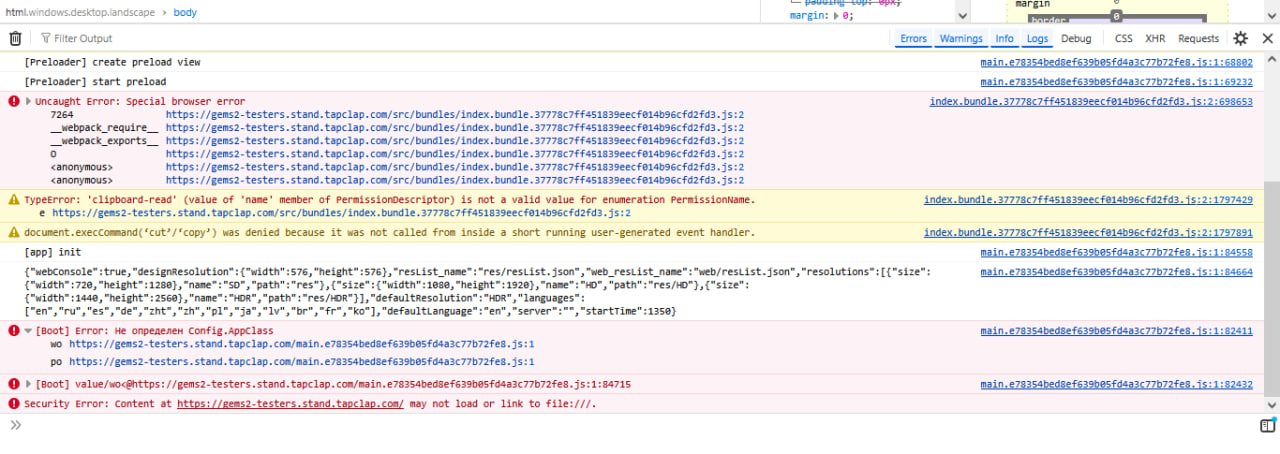
\includegraphics[width=1\linewidth,height=\textheight,keepaspectratio,alt={desktop}]{assets/firefox-startup-1.jpg}
\caption{desktop}\label{fig:firefox-startup-1}
\end{figure}

\begin{figure}
\centering

\includegraphics[width=1\linewidth,height=\textheight,keepaspectratio,alt={desktop}]{assets/firefox-startup-2.jpg}
\caption{desktop}\label{fig:firefox-startup-2}
\end{figure}

\begin{figure}
\centering

\includegraphics[width=1\linewidth,height=\textheight,keepaspectratio,alt={Android}]{assets/firefox-startup-3.jpg}
\caption{Android}\label{fig:firefox-startup-3}
\end{figure}

\clearpage

\subsubsection{BUG-02. Game freezes during level transition: board
remains visible and input becomes
unresponsive}\label{bug-02.-game-freezes-during-level-transition-board-remains-visible-and-input-becomes-unresponsive}

\textbf{issues:}
\href{https://github.com/Dubinetsky/tapclap/issues/2}{Game freezes
during level transition: board remains visible and input becomes
unresponsive}

Наблюдалось Оксаной Дубинецкой во время ручного тестирования на
компьютере, впоследствии повторно воспроизведено во время
автоматизированного прогона с помощью
\href{WARDEN}{https://github.com/pan-canon/TheWorldOfCanon/tree/main/work/tapclap/warden}.

\textbf{Окружение:}

\begin{itemize}
\tightlist
\item
  Desktop Google Chrome
\item
  Тестовая сборка: Pirate Treasures
\item
  Engine: Cocos2d-JS v3.17
\item
  Environment: test
\item
  Игровое поле: 7×7
\end{itemize}

\textbf{Наблюдаемое поведение:}

При прохождении уровня ближе к его завершению игровое поле перестаёт
реагировать на действия пользователя.

Визуально поле остаётся на экране, однако дальнейшие перестановки фишек
не выполняются, а ожидаемый переход к следующему состоянию игры не
завершается.

Проблема первоначально была воспроизведена вручную, а затем повторно во
время автоматизированного прогона с помощью WARDEN.

До возникновения зависания WARDEN корректно определял поле как полную и
читаемую сетку 7×7 с шестью типами фишек.

\textbf{Шаги воспроизведения:}

\begin{enumerate}
\def\labelenumi{\arabic{enumi}.}
\tightlist
\item
  Открыть тестовую версию игры в Chrome.
\item
  Начать уровень и выполнять допустимые ходы.
\item
  Продолжать игру до состояния, близкого к завершению уровня.
\item
  Наблюдать состояние игры после очередного хода.
\item
  Попытаться выполнить следующий ход на поле.
\end{enumerate}

\newpage

Для повторного автоматизированного воспроизведения использовался WARDEN:

\begin{Shaded}
\begin{Highlighting}[]
\BuiltInTok{window}\OperatorTok{.}\AttributeTok{warden} \OperatorTok{=} \ControlFlowTok{await}\NormalTok{ WARDEN}\OperatorTok{.}\FunctionTok{init}\NormalTok{(\{}
  \DataTypeTok{rows}\OperatorTok{:} \DecValTok{7}\OperatorTok{,}
  \DataTypeTok{cols}\OperatorTok{:} \DecValTok{7}\OperatorTok{,}
  \DataTypeTok{cellSize}\OperatorTok{:} \DecValTok{72}\OperatorTok{,}
  \DataTypeTok{expectedTypes}\OperatorTok{:} \DecValTok{6}
\NormalTok{\})}\OperatorTok{;}
\end{Highlighting}
\end{Shaded}

Контрольный короткий прогон:

\begin{Shaded}
\begin{Highlighting}[]
\ControlFlowTok{await}\NormalTok{ warden}\OperatorTok{.}\FunctionTok{run}\NormalTok{(\{ }\DataTypeTok{maxSteps}\OperatorTok{:} \DecValTok{10}\NormalTok{ \})}\OperatorTok{;}
\end{Highlighting}
\end{Shaded}

Длинный прогон:

\begin{Shaded}
\begin{Highlighting}[]
\ControlFlowTok{await}\NormalTok{ warden}\OperatorTok{.}\FunctionTok{run}\NormalTok{(\{ }\DataTypeTok{maxSteps}\OperatorTok{:} \DecValTok{50}\NormalTok{ \})}\OperatorTok{;}
\end{Highlighting}
\end{Shaded}

\textbf{Ожидаемое поведение:}

После выполнения условий уровня игра должна корректно завершить текущее
игровое состояние и перейти к следующему экрану или состоянию.

Поле не должно оставаться визуально активным в состоянии, когда
пользовательский ввод больше не обрабатывается.

\textbf{Сравнение:}

Короткий контрольный прогон из 10 последовательных допустимых ходов
проходит полностью: каждый ход завершается изменением состояния поля.

\begin{Shaded}
\begin{Highlighting}[]
\NormalTok{[WARDEN] RUN START \{maxSteps: 10\}}
\NormalTok{[WARDEN] PASS BOARD\_CHANGED}
\NormalTok{[WARDEN] PASS BOARD\_CHANGED}
\NormalTok{...}
\NormalTok{[WARDEN] RUN FINISHED}
\end{Highlighting}
\end{Shaded}

Все 10 ходов контрольного прогона завершились успешно.

\newpage

Во время более длинного прогона также выполняется продолжительная
последовательность допустимых ходов:

\begin{Shaded}
\begin{Highlighting}[]
\NormalTok{[WARDEN] RUN START \{maxSteps: 50\}}
\NormalTok{[WARDEN] perform \{...\}}
\NormalTok{[WARDEN] PASS BOARD\_CHANGED}
\NormalTok{[WARDEN] perform \{...\}}
\NormalTok{[WARDEN] PASS BOARD\_CHANGED}
\NormalTok{...}
\end{Highlighting}
\end{Shaded}

После очередного хода WARDEN перестаёт получать стабильное читаемое
состояние поля и завершает ожидание по таймауту:

\begin{Shaded}
\begin{Highlighting}[]
\NormalTok{[WARDEN] RUN STOP \{}
\NormalTok{  status: \textquotesingle{}ERROR\textquotesingle{},}
\NormalTok{  error: \textquotesingle{}Error: WARDEN: board did not reach a stable readable state\textquotesingle{}}
\NormalTok{\}}
\end{Highlighting}
\end{Shaded}

После возникновения зависания повторное чтение обычного игрового поля
также становится невозможным:

\begin{Shaded}
\begin{Highlighting}[]
\NormalTok{Uncaught Error: WARDEN: gem layer not found for 7x7}
\NormalTok{    at discoverGemLayer}
\NormalTok{    at Object.read}
\end{Highlighting}
\end{Shaded}

При этом сама Cocos-сцена продолжает существовать: в scene graph
остаются видимые и активные (\texttt{visible:\ true},
\texttt{running:\ true}) игровые узлы. Визуально поле также остаётся на
экране.

\textbf{Текущая интерпретация:}

После перезагрузки страницы игра загружается уже в последующем состоянии
прогресса: появляются дальнейшие задания и контент.

Это позволяет предположить, что проблема возникает во время клиентского
перехода между состояниями уровня: прогресс уже может быть обработан,
тогда как визуальное состояние не завершает переход корректно.

До зависания слой игрового поля определялся в scene graph как:

\begin{Shaded}
\begin{Highlighting}[]
\NormalTok{scene/Class[0]/gameViewLayer[6]/Class[0]/Class[3]}
\end{Highlighting}
\end{Shaded}

и содержал читаемую сетку 7×7.

После зависания структура scene graph изменяется, и WARDEN больше не
может определить стандартный слой игрового поля, хотя остальные узлы
сцены продолжают работать.

Это согласуется с гипотезой о незавершённом переходе игрового состояния,
но не доказывает конкретную внутреннюю причину дефекта.

\textbf{Статус:}

Обнаружено вручную. Повторно воспроизведено автоматизированным прогоном
WARDEN.

\textbf{Источник наблюдения:}

\texttt{{[}Manual{]}\ {[}WARDEN{]}\ {[}DevTools{]}}

\textbf{Доказательства:}

\begin{itemize}
\tightlist
\item
  Ручное воспроизведение зависания;
\item
  Повторное воспроизведение во время длинного WARDEN-прогона;
\item
  Успешный контрольный прогон из 10 последовательных ходов;
\item
  Лог остановки по
  \texttt{board\ did\ not\ reach\ a\ stable\ readable\ state};
\item
  Последующая ошибка \texttt{gem\ layer\ not\ found\ for\ 7x7};
\item
  Наблюдение scene graph до и после зависания;
\item
  Скриншот игрового поля в зависшем состоянии;
\item
  runtime-лог Cocos2d-JS v3.17.
\end{itemize}

Конфигурация runtime подтверждает тестовое окружение:
\texttt{production:\ false}, \texttt{market:\ "test"}.

\newpage

\subsection{2. Приведите примеры тестирования методом граничных значений
в нашей
игре}\label{ux43fux440ux438ux432ux435ux434ux438ux442ux435-ux43fux440ux438ux43cux435ux440ux44b-ux442ux435ux441ux442ux438ux440ux43eux432ux430ux43dux438ux44f-ux43cux435ux442ux43eux434ux43eux43c-ux433ux440ux430ux43dux438ux447ux43dux44bux445-ux437ux43dux430ux447ux435ux43dux438ux439-ux432-ux43dux430ux448ux435ux439-ux438ux433ux440ux435}

Метод граничных значений --- это проверка значений непосредственно на
границе допустимого диапазона и рядом с ней: обычно N−1, N, N+1. Именно
в таких переходных состояниях часто проявляются ошибки.

Примеры для игры:

\begin{enumerate}
\def\labelenumi{\arabic{enumi}.}
\tightlist
\item
  \textbf{Оставшиеся ходы на уровне:} проверить состояния с 2, 1 и 0
  ходами. Особенно важен последний ход: сначала должны полностью
  обработаться созданная комбинация и возможные каскады, и только затем
  игра должна определить победу или поражение.
\item
  \textbf{Счётчик цели уровня:} если осталось собрать 2, 1 и 0 объектов,
  проверить корректность уменьшения счётчика. При достижении 0 уровень
  должен завершиться один раз, а значение не должно уходить в
  отрицательное.
\item
  \textbf{Количество доступных ходов на поле:} проверить состояния с 0,
  1 и несколькими допустимыми ходами. При одном допустимом ходе
  подсказка должна указывать на него; при отсутствии ходов игра должна
  корректно обработать это состояние, например выполнить перемешивание,
  если такая механика предусмотрена.
\item
  \textbf{Границы игрового поля:} проверить перестановки на первой и
  последней строке, первом и последнем столбце и в углах. Попытка свайпа
  за пределы поля не должна приводить к некорректному обмену, ошибке или
  зависанию.
\item
  \textbf{Порог открытия механики или контента:} если функция становится
  доступна с уровня N, проверить N−1, N и N+1: до порога она должна быть
  недоступна, на самом пороге открыться, а после него оставаться
  доступной.
\end{enumerate}

Отдельно важен переход из состояния «цель ещё не выполнена» в состояние
«цель выполнена», особенно если это происходит последним ходом. В этот
момент одновременно меняются состояние поля, результат уровня и
интерфейс следующего экрана.

Во время тестирования как раз был обнаружен дефект на такой границе:
после завершения игрового состояния поле оставалось отображённым, но
переставало принимать ввод и ожидаемый переход дальше не завершался. Сам
по себе этот дефект относится к функциональному тестированию, но момент
его возникновения является хорошим примером того, почему граничные
переходы нужно проверять отдельно.

\newpage

\subsection{3. После крупного обновления упала производительность
Android-версии
игры}\label{ux43fux43eux441ux43bux435-ux43aux440ux443ux43fux43dux43eux433ux43e-ux43eux431ux43dux43eux432ux43bux435ux43dux438ux44f-ux443ux43fux430ux43bux430-ux43fux440ux43eux438ux437ux432ux43eux434ux438ux442ux435ux43bux44cux43dux43eux441ux442ux44c-android-ux432ux435ux440ux441ux438ux438-ux438ux433ux440ux44b}

\begin{quote}
Ваш руководитель и коллеги по отделу QA в отпуске. После крупного
обновления в четверг массово поступают жалобы от пользователей, что
упала производительность android-версии игры. Вы узнаете об этому в
пятницу утром. Времени мало, откатить версию нет возможности,
программисты ждут информации и локализации проблемы. Составьте,
пожалуйста, чек-лист ваших действий в приоритетном порядке.
\end{quote}

В такой ситуации моя первая задача --- как можно быстрее не просто
подтвердить проблему, а сузить её до конкретного сценария, устройства
или изменения, чтобы разработчики могли начать работу.

\begin{enumerate}
\def\labelenumi{\arabic{enumi}.}
\tightlist
\item
  Просмотреть обращения пользователей и сгруппировать симптомы: падение
  FPS, долгие загрузки, фризы, зависания, нагрев, повышенный расход
  батареи и т. д. Отдельно отметить модели устройств, версии Android и
  игровые сценарии, которые повторяются чаще всего.
\item
  Уточнить, действительно ли проблема появилась после последнего
  обновления, и посмотреть, какие подсистемы или ресурсы менялись в этом
  релизе.
\item
  Попробовать быстро воспроизвести проблему на нескольких
  Android-устройствах: сначала на конфигурациях, которые чаще всего
  встречаются в жалобах, затем на контрольном устройстве.
\item
  Сузить сценарий воспроизведения: определить, возникает ли деградация
  при запуске, на карте, во время уровня, при каскадах и эффектах, после
  рекламы, при переходах между экранами или после длительной сессии.
\item
  Зафиксировать измеримые показатели: FPS/frame time, время загрузки,
  использование CPU, RAM и GPU, возможный рост памяти, нагрев и сетевую
  активность. Если доступны, использовать Android Vitals, Firebase
  Performance/Crashlytics, Android Profiler, Perfetto или adb.
\item
  Проверить зависимости: модель устройства и GPU, версия Android,
  разрешение экрана, графические настройки, сеть, продолжительность
  сессии, конкретный уровень или новая механика.
\item
  Если доступна предыдущая сборка, сравнить тот же сценарий на ней.
  Production откатывать нельзя, но старая APK может быть полезна как
  контроль для локализации регрессии.
\item
  Как только появляется устойчивое воспроизведение, сразу передать
  разработчикам минимальный пакет: build, устройство, Android version,
  шаги, expected/actual result, частоту воспроизведения, видео, логи и
  метрики. Не ждать окончания полного исследования, если информации уже
  достаточно для начала исправления.
\item
  Параллельно проверять гипотезы разработчиков и уточнять область
  проблемы.
\item
  После исправления проверить fix именно на проблемных конфигурациях и
  выполнить короткий performance regression smoke по основным игровым
  сценариям.
\end{enumerate}

\newpage

\subsection{4. Чек-лист проверки бонусного мира «Знакомство с
пиратом»}\label{ux447ux435ux43a-ux43bux438ux441ux442-ux43fux440ux43eux432ux435ux440ux43aux438-ux431ux43eux43dux443ux441ux43dux43eux433ux43e-ux43cux438ux440ux430-ux437ux43dux430ux43aux43eux43cux441ux442ux432ux43e-ux441-ux43fux438ux440ux430ux442ux43eux43c}

\begin{quote}
В тестовой версии игры есть бонусный мир ``Знакомство с пиратом''.
Основываясь на своем опыте из первого задания, напишите чек-лист для
проверки этого бонусного мира.
\end{quote}

Во время проверки я прошла первые три уровня бонусного мира и
использовала фактически встреченные состояния как основу чек-листа.

\begin{enumerate}
\def\labelenumi{\arabic{enumi}.}
\tightlist
\item
  Проверить вход в бонусный мир с основной карты по кораблю.
\item
  Проверить корректность первого tutorial-состояния: затемнение фона,
  реплика персонажа, указатель на нужный элемент, блокировка лишних
  действий.
\item
  Проверить открытие карточки уровня: номер уровня, цель,
  доступные/заблокированные элементы, кнопки Play и X.
\item
  Проверить запуск уровня после нажатия Play.
\item
  Проверить отображение цели уровня и исходного количества ходов.
\item
  Проверить tutorial внутри уровня: подсказка должна показывать
  допустимое действие и не приводить игру в некорректное состояние при
  попытке нажать или свайпнуть в другом месте.
\item
  Проверить базовые match-3 действия: допустимый swap, недопустимый
  swap, каскады и заполнение освободившихся клеток.
\item
  Проверить специальные комбинации, которым обучает бонусный мир, и
  соответствие результата показанной подсказке.
\item
  Проверить изменение счётчика цели после уничтожения необходимых
  объектов.
\item
  Проверить уменьшение числа ходов и граничные состояния 2, 1, 0.
\item
  Проверить завершение уровня при выполнении цели.
\item
  Проверить экран Level completed: количество звёзд, очки, кнопки Next,
  Share, X.
\item
  Проверить переход на следующий уровень через Next.
\item
  Проверить последовательное открытие уровней и отсутствие возможности
  начать ещё заблокированный уровень раньше времени.
\item
  Проверить накопительный прогресс бонусного мира/сундука после
  прохождения уровней.
\item
  Проверить повторный вход в бонусный мир после выхода на основную
  карту.
\item
  Проверить сохранение прогресса после перезагрузки страницы или
  перезапуска игры.
\item
  Проверить поражение при окончании ходов без выполнения цели и
  возможность повторного запуска уровня.
\item
  Проверить закрытие карточки уровня и экрана завершения через X, а
  также возврат в ожидаемое предыдущее состояние.
\item
  Проверить несколько быстрых последовательных нажатий на Play, Next, X,
  чтобы исключить двойной запуск уровня или наложение экранов.
\item
  Проверить, что после нескольких пройденных уровней счётчики, награды и
  состояние карты не сбрасываются и не дублируются.
\item
  Повторить основные проверки на мобильном устройстве: масштабирование
  UI, tap/swipe, читаемость tutorial, ориентация экрана и отсутствие
  перекрывающихся элементов.
\end{enumerate}

Отдельное внимание я бы уделила переходам между состояниями: запуск
уровня, завершение цели, экран результата, Next и возврат на карту. В
основном игровом сценарии уже был найден дефект именно на переходе после
завершения уровня, поэтому аналогичные точки в бонусном мире считаю
повышенно рискованными.

\newpage

\subsection{5. Напишите тест-кейс(ы) (не более 10) на проверку уровня
и/или любой игровой механики из нашей
игры.}\label{ux43dux430ux43fux438ux448ux438ux442ux435-ux442ux435ux441ux442-ux43aux435ux439ux441ux44b-ux43dux435-ux431ux43eux43bux435ux435-10-ux43dux430-ux43fux440ux43eux432ux435ux440ux43aux443-ux443ux440ux43eux432ux43dux44f-ux438ux438ux43bux438-ux43bux44eux431ux43eux439-ux438ux433ux440ux43eux432ux43eux439-ux43cux435ux445ux430ux43dux438ux43aux438-ux438ux437-ux43dux430ux448ux435ux439-ux438ux433ux440ux44b.}

Для повторяемых проверок я вынесла восемь сценариев в WARDEN. Они
используют одно и то же ядро чтения состояния поля и ввода, поэтому в
самих кейсах не дублируется обход scene graph или логика взаимодействия
с canvas.

\subsubsection{TC-01. Допустимая
перестановка}\label{tc-01.-ux434ux43eux43fux443ux441ux442ux438ux43cux430ux44f-ux43fux435ux440ux435ux441ux442ux430ux43dux43eux432ux43aux430}

\textbf{Что проверяет:} WARDEN находит допустимый match-3 ход,
отправляет его в игру и проверяет, что после завершения анимации
логическое состояние поля изменилось.

\textbf{Ожидаемый результат:} существует хотя бы один legal move; после
его выполнения поле отличается от исходного.

\textbf{Автоматизированный сценарий}:
\href{../scenarios/TC-01-valid-swap-snippet.js}{https://github.com/Dubinetsky/tapclap/blob/main/scenarios/TC-01-valid-swap-snippet.js}.

\subsubsection{TC-02. Недопустимая
перестановка}\label{tc-02.-ux43dux435ux434ux43eux43fux443ux441ux442ux438ux43cux430ux44f-ux43fux435ux440ux435ux441ux442ux430ux43dux43eux432ux43aux430}

\textbf{Что проверяет:} WARDEN выбирает соседнюю пару, которая по
независимому solver не создаёт match-3, и выполняет обмен.

\textbf{Ожидаемый результат:} после возможной reject-анимации итоговое
состояние поля совпадает с исходным; недопустимый swap не должен менять
доску.

\textbf{Автоматизированный сценарий:}
\href{../scenarios/TC-02-invalid-swap-snippet.js}{https://github.com/Dubinetsky/tapclap/blob/main/scenarios/TC-02-invalid-swap-snippet.js}.

\subsubsection{TC-03. Каскад и заполнение
поля}\label{tc-03.-ux43aux430ux441ux43aux430ux434-ux438-ux437ux430ux43fux43eux43bux43dux435ux43dux438ux435-ux43fux43eux43bux44f}

\textbf{Что проверяет:} выполняется один допустимый ход, после чего
WARDEN ждёт окончания каскадов и refill.

\textbf{Ожидаемый результат:} после завершения всех анимаций поле снова
читается как полная и стабильная сетка. Сценарий не считает количество
каскадов, а проверяет возвращение игры в корректное читаемое состояние.

\textbf{Автоматизированный сценарий}:
\href{../scenarios/TC-03-cascade-refill-snippet.js}{https://github.com/Dubinetsky/tapclap/blob/main/scenarios/TC-03-cascade-refill-snippet.js}.

\subsubsection{TC-04. Проверка штатной
подсказки}\label{tc-04.-ux43fux440ux43eux432ux435ux440ux43aux430-ux448ux442ux430ux442ux43dux43eux439-ux43fux43eux434ux441ux43aux430ux437ux43aux438}

\textbf{Что проверяет}: без взаимодействия с полем WARDEN ждёт штатную
hint-анимацию и пытается определить подсказанную пару клеток по
публичным свойствам Nodes. Затем эта пара сравнивается с независимо
рассчитанным списком legal moves.

\textbf{Ожидаемый результат:}

\begin{itemize}
\tightlist
\item
  \texttt{VALID\_HINT} --- подсказка соответствует допустимому ходу;
\item
  \texttt{INVALID\_HINT} --- подсказка не входит в список допустимых
  ходов и является кандидатом на дефект;
\item
  \texttt{AMBIGUOUS} --- наблюдатель не смог уверенно распознать
  анимацию, но такой результат не считается провалом игры.
\end{itemize}

\textbf{Автоматизированный сценарий:}
\href{../scenarios/TC-04-hint-validation-snippet.js}{https://github.com/Dubinetsky/tapclap/blob/main/scenarios/TC-04-hint-validation-snippet.js}.

\subsubsection{TC-05. Несколько последовательных допустимых
ходов}\label{tc-05.-ux43dux435ux441ux43aux43eux43bux44cux43aux43e-ux43fux43eux441ux43bux435ux434ux43eux432ux430ux442ux435ux43bux44cux43dux44bux445-ux434ux43eux43fux443ux441ux442ux438ux43cux44bux445-ux445ux43eux434ux43eux432}

\textbf{Что проверяет:} WARDEN выполняет десять последовательных
допустимых ходов. После каждого хода реальное состояние поля считывается
заново, а legal moves пересчитываются уже для новой позиции.

\textbf{Ожидаемый результат}: все десять шагов завершаются со статусом
\texttt{MOVED}; очередь ходов не строится заранее, потому что каскад и
refill изменяют состояние поля.

\textbf{Автоматизированный сценарий:}
\href{../scenarios/TC-05-repeated-play-snippet.js}{https://github.com/Dubinetsky/tapclap/blob/main/scenarios/TC-05-repeated-play-snippet.js}.

\subsubsection{TC-06. Стабильность чтения
поля}\label{tc-06.-ux441ux442ux430ux431ux438ux43bux44cux43dux43eux441ux442ux44c-ux447ux442ux435ux43dux438ux44f-ux43fux43eux43bux44f}

\textbf{Что проверяет:} после \texttt{waitStable()} WARDEN дважды
считывает игровую матрицу с небольшой паузой.

\textbf{Ожидаемый результат:} оба чтения полные, а логическая матрица
между ними не меняется. Этот кейс проверяет пригодность board reader как
основы для остальных автоматизированных сценариев.

\textbf{Автоматизированный сценарий:}
\href{../scenarios/TC-06-board-stability-snippet.js}{https://github.com/Dubinetsky/tapclap/blob/main/scenarios/TC-06-board-stability-snippet.js}.

\subsubsection{TC-07. Блокировка
ввода}\label{tc-07.-ux431ux43bux43eux43aux438ux440ux43eux432ux43aux430-ux432ux432ux43eux434ux430}

\textbf{Что проверяет:} WARDEN последовательно выполняет допустимые ходы
и ищет состояние, при котором независимый solver видит legal move,
корректный drag отправлен в игру, но итоговое состояние поля не
изменилось.

\textbf{Ожидаемый результат:} если блокировка не воспроизводится,
сценарий завершается как \texttt{NOT\ REPRODUCED}. Если состояние
найдено, WARDEN сохраняет диагностический snapshot, конкретный ход и
состояние доски. Сам сценарий не объявляет root cause.

\textbf{Автоматизированный сценарий:}
\href{../scenarios/TC-07-input-lock-snippet.js}{https://github.com/Dubinetsky/tapclap/blob/main/scenarios/TC-07-input-lock-snippet.js}.

\subsubsection{TC-08. Переход после завершения
уровня}\label{tc-08.-ux43fux435ux440ux435ux445ux43eux434-ux43fux43eux441ux43bux435-ux437ux430ux432ux435ux440ux448ux435ux43dux438ux44f-ux443ux440ux43eux432ux43dux44f}

\textbf{Что проверяет:} WARDEN продолжает выполнять допустимые ходы до
одного из условий остановки: игровая сетка исчезла или сменилась сцена,
закончились legal moves, обнаружена блокировка ввода либо достигнут
защитный лимит ходов.

\textbf{Ожидаемый результат:} исчезновение обычной сетки трактуется
только как кандидат на переход уровня. Финальное окно или экран
завершения уровня после этого проверяется вручную. Если поле не
реагирует на legal move, сценарий сохраняет соответствующее
диагностическое состояние.

\textbf{Автоматизированный сценарий:}
\href{../scenarios/TC-08-level-completion-snippet.js}{https://github.com/Dubinetsky/tapclap/blob/main/scenarios/TC-08-level-completion-snippet.js}.

\newpage

\subsection{6. Игроки стали часто проигрывать на 10-м уровне, но среднее
число использованных ходов почти не изменилось. Предложите не менее трёх
возможных причин и способы их
проверки}\label{ux438ux433ux440ux43eux43aux438-ux441ux442ux430ux43bux438-ux447ux430ux441ux442ux43e-ux43fux440ux43eux438ux433ux440ux44bux432ux430ux442ux44c-ux43dux430-10-ux43c-ux443ux440ux43eux432ux43dux435-ux43dux43e-ux441ux440ux435ux434ux43dux435ux435-ux447ux438ux441ux43bux43e-ux438ux441ux43fux43eux43bux44cux437ux43eux432ux430ux43dux43dux44bux445-ux445ux43eux434ux43eux432-ux43fux43eux447ux442ux438-ux43dux435-ux438ux437ux43cux435ux43dux438ux43bux43eux441ux44c.-ux43fux440ux435ux434ux43bux43eux436ux438ux442ux435-ux43dux435-ux43cux435ux43dux435ux435-ux442ux440ux451ux445-ux432ux43eux437ux43cux43eux436ux43dux44bux445-ux43fux440ux438ux447ux438ux43d-ux438-ux441ux43fux43eux441ux43eux431ux44b-ux438ux445-ux43fux440ux43eux432ux435ux440ux43aux438}

Сам факт, что среднее число использованных ходов почти не изменилось,
означает, что сначала я бы не делала вывод о нехватке ходов. Игроки
по-прежнему тратят примерно столько же действий, но результат этих
действий мог стать хуже. Также среднее значение может скрывать изменения
внутри отдельных групп игроков.

\begin{enumerate}
\def\labelenumi{\arabic{enumi}.}
\item
  \textbf{Уровень стал объективно сложнее при том же количестве ходов?}

  Например, могла измениться цель уровня, количество препятствий,
  расположение элементов или вероятность появления нужных фишек.

  \textbf{Как проверить:} сравнить текущую конфигурацию 10-го уровня с
  предыдущей версией + несколько раз пройти уровень на обеих сборках +
  сравнить win rate, число выполненных целей к последнему ходу и
  распределение оставшихся невыполненных целей.
\item
  \textbf{Изменилась генерация или перемешивание игрового поля?}

  Количество ходов остаётся тем же, но игроку чаще попадаются менее
  выгодные стартовые позиции, меньше доступных комбинаций или хуже
  формируются специальные элементы.

  \textbf{Как проверить:} собрать выборку стартовых полей и игровых
  сессий до и после изменения + сравнить количество доступных ходов,
  частоту reshuffle, количество каскадов и создаваемых специальных
  комбинаций. Дополнительно можно автоматически прогнать большое число
  состояний независимым solver.
\item
  \textbf{Какая-либо механика перестала работать или стала работать
  иначе?}

  Например, комбинация уничтожает меньше объектов, цель не всегда
  засчитывается, специальная фишка действует неправильно или часть
  результата каскада теряется.

  \textbf{Как проверить:} воспроизвести основные механики 10-го уровня
  отдельно и проверить изменение счётчиков после каждого действия.
  Сопоставить визуальный результат на поле с фактическим прогрессом
  цели.
\item
  \textbf{Изменился состав игроков, дошедших до 10-го уровня?}

  После обновления или изменения ранних уровней до него могла начать
  доходить другая аудитория: например, больше новых игроков, которые
  хуже знают механику.

  \textbf{Как проверить:} сегментировать статистику по новым и
  возвращающимся игрокам, версии клиента, дате установки, платформе и
  другим доступным признакам. Сравнить win rate внутри одинаковых
  когорт, а не только общий показатель.
\item
  \textbf{Среднее количество ходов скрывает изменение распределения?}

  Например, раньше часть игроков выигрывала за 15 ходов, а часть
  проигрывала за 25, а теперь почти все доходят до последних ходов и
  чаще проигрывают. Среднее при этом может измениться совсем немного.

  \textbf{Как проверить:} посмотреть не только среднее, но и медиану,
  распределение использованных ходов, а также отдельно среднее для побед
  и поражений. Дополнительно сравнить, на каком ходу чаще всего
  завершается успешная и неуспешная попытка.
\end{enumerate}

В первую очередь я бы проверила изменения самого уровня и игровых
механик, потому что рост проигрышей при примерно неизменном количестве
ходов больше похож на снижение эффективности каждого хода, чем просто на
изменение лимита ходов.

\newpage

\subsection{7. Опишите, как бы вы обучили игрока новой механике, не
используя длинные текстовые
инструкции}\label{ux43eux43fux438ux448ux438ux442ux435-ux43aux430ux43a-ux431ux44b-ux432ux44b-ux43eux431ux443ux447ux438ux43bux438-ux438ux433ux440ux43eux43aux430-ux43dux43eux432ux43eux439-ux43cux435ux445ux430ux43dux438ux43aux435-ux43dux435-ux438ux441ux43fux43eux43bux44cux437ux443ux44f-ux434ux43bux438ux43dux43dux44bux435-ux442ux435ux43aux441ux442ux43eux432ux44bux435-ux438ux43dux441ux442ux440ux443ux43aux446ux438ux438}

Я бы обучала через сам геймплей по принципу:

показать \textgreater\textgreater{} дать попробовать
\textgreater\textgreater{} проверить понимание
\textgreater\textgreater{} усложнить

Сначала я бы поставила игрока в безопасную ситуацию, где новая механика
очевидно полезна и почти невозможно ошибиться. Нужный объект или
действие подсвечиваются визуально, а интерфейс даёт короткую контекстную
подсказку --- например, иконку кнопки вместо длинного текста. После
первого действия игрок сразу получает понятный feedback: анимацию, звук
или изменение состояния мира.

Дальше я бы дала похожую ситуацию уже без явной подсказки, чтобы игрок
самостоятельно повторил действие. После этого механику можно постепенно
сочетать с уже знакомыми системами и повышать сложность. Таким образом
обучение происходит через контролируемую последовательность игровых
ситуаций, а не через длинное объяснение правил.

\newpage

\subsection{8. Семидневный ивент из 30 этапов: длительность и
распределение
наград}\label{ux441ux435ux43cux438ux434ux43dux435ux432ux43dux44bux439-ux438ux432ux435ux43dux442-ux438ux437-30-ux44dux442ux430ux43fux43eux432-ux434ux43bux438ux442ux435ux43bux44cux43dux43eux441ux442ux44c-ux438-ux440ux430ux441ux43fux440ux435ux434ux435ux43bux435ux43dux438ux435-ux43dux430ux433ux440ux430ux434}

Ивент длится семь дней и состоит из 30 этапов. Определите, сколько
времени активному игроку потребуется для его завершения, и предложите
распределение наград.

Без данных о средней длительности этапа и проценте повторных попыток
точное время определить нельзя, поэтому сначала задам рабочее допущение.

Если один этап занимает в среднем 5--6 минут, а часть сложных этапов
требует повторного прохождения, то 30 этапов займут примерно 3--4 часа
чистого игрового времени.

Для семидневного ивента я бы ориентировалась на такой темп:

\begin{itemize}
\tightlist
\item
  Примерно 4--5 этапов в день;
\item
  Около 25--35 минут активной игры в день;
\item
  Активный игрок сможет закончить ивент примерно за 5--6 дней, оставив
  последний день как запас на пропущенную сессию или сложные этапы.
\end{itemize}

Мне кажется важным, чтобы обязательный ежедневный объём не требовал от
игрока проходить событие по часу в день: ивент должен мотивировать
регулярно возвращаться, но не превращаться в отдельную работу.

Распределение наград:

\begin{enumerate}
\def\labelenumi{\arabic{enumi}.}
\tightlist
\item
  Каждый этап --- небольшая гарантированная награда, чтобы прохождение
  всегда давало видимый прогресс.
\item
  Каждый 5-й этап --- более заметная milestone-награда: этапы 5, 10, 15,
  20 и 25.
\item
  Этап 30 --- главная награда события: наиболее редкий или ценный приз.
\item
  Общую ценность наград я бы постепенно увеличивала к концу события:
  первые этапы дают быстрый положительный feedback, а последние создают
  мотивацию завершить весь ивент.
\item
  Примерно 50--60\% общей ценности наград можно распределить по обычным
  этапам и промежуточным milestone, а оставшиеся 40--50\% оставить на
  последние milestone и финальную награду.
\item
  Я бы не концентрировала почти всю ценность только на 30-м этапе:
  игрок, который активно участвовал, но не успел пройти последние
  несколько этапов, всё равно должен получить ощутимую награду за
  потраченное время.
\end{enumerate}

Дополнительно я бы проверила баланс по реальным данным после запуска:
среднее время этапа, число попыток, процент игроков, дошедших до этапов
5/10/15/20/25/30, и точки, на которых игроки чаще всего прекращают
участие. Если большинство активных игроков не успевает закончить 30
этапов за 7 дней, сложность или требуемое игровое время стоит уменьшить.

\end{document}